\section{Generative Models}
Generative models aim to learn the underlying probability distribution of data, enabling them to generate 
new samples that closely resemble those in the training set. Unlike discriminative models, which focus on 
modeling the conditional probability $p(y|x)$ to find decision boundaries between classes,  generative models
learn the joint distribution $p(x,y)$, typically by modeling $p(x|y)$  along with the class prior $p(y)$.
Additionally, once trained, generative models can be employed for classification tasks using Bayes' theorem:
$$p(y|x) = \frac{p(x|y)p(y)}{p(x)} = \frac{p(x|y)p(y)}{\sum_{y}p(x|y)p(y)} $$

\subsection{Autoencoders}
Autoencoders (AEs) are a type of neural network used for unsupervised learning, specifically for learning a compressed, 
efficient representation (encoding) of data. An autoencoder consists of two main parts:

\begin{enumerate}
    \item \textbf{Encoder}: This part takes the input data $x$ and maps it to a lower-
    dimensional space, often referred to as the latent space or embedding space. The 
    encoder produces an encoded representation $z = f(x)$
    
    \item \textbf{Decoder}: The decoder takes this compressed representation $z$ and tries 
    to reconstruct the original input $x'$ from it. The goal is to minimize the difference 
    between the input $x$ and the reconstructed output $x'$.
\end{enumerate}

The autoencoder is trained to minimize the reconstruction error, meaning it learns to 
represent the data in a lower-dimensional space while still being able to recover the 
original data as closely as possible.\newline 
While autoencoders are good at learning compact representations of data, they are not 
inherently designed for generative modeling. The problem is that the encoding learned by 
the autoencoder might not be structured in a way that facilitates easy sampling and 
generation. In other words, the latent space may not have meaningful properties (such as 
smoothness or continuity) that are useful for generating new data.

\subsection{Variational Autoencoders (VAEs)}
To address these limitations, Variational Autoencoders (VAEs) were introduced. VAEs are a 
probabilistic extension of autoencoders that are designed specifically for generative 
modeling. While AEs learn deterministic encodings, VAEs learn probabilistic encodings and 
allow for sampling from a continuous latent space. They work as follows :

\begin{enumerate}
    \item \textbf{Encoder}: In a VAE, the encoder outputs two vectors: the mean $\mu(x)$ and the standard deviation
    $\sigma(x)$  of a distribution (often a Gaussian distribution) in the latent space. Instead of producing a single 
    point in the latent space like in regular autoencoders, VAEs learn a distribution over the latent space.
    The encoder approximates the posterior distribution $p(z|x) \approx q_\psi(z|x)$.% While the latent space is just a normal distribution  $\mathcal{N}(0,1)$.
    \item \textbf{Reparameterization Trick}: To sample from this distribution in a 
    differentiable way (which is required for backpropagation), VAEs use the reparameterization trick \ref{reparametrization_trick}. 
    The trick ensures that the gradient can flow 
    through the random sampling process by expressing the latent variable $z$ as: $$z = 
    \mu(x)+\sigma(x) \cdot \epsilon$$ where $\epsilon$ is a random noise sampled from a 
    standard normal distribution (usually $\mathcal{N}(0,1)$)
    \item \textbf{Decoder}: After sampling from the distribution, the decoder reconstructs the input $x'$ from the sampled 
    latent variable $z$ as in a standard autoencoder.
\end{enumerate}
In VAEs the prior is chosen to be a standard multivariate normal distribution $p(z) \sim \mathcal{N}(0,I)$. The VAE is trained 
using maximum likelihood estimation
\begin{align*}
   \log{p_\theta(x)} &= \log{\int p_\theta(z,x)} \mathrm{d}z && \text{(marginalization)} \\
   &= \log{ \int \frac{q_\psi(z|x)}{q_\psi(z|x)} p_\theta(z,x)} \mathrm{d}z \\
   &= \log{\underset{z \sim q_\psi(z|x)}{\mathbb{E}}\left[\frac{p_\theta(z,x)} {q_\psi(z|x)}\right]} \\
   &\geq  \underset{z \sim q_\psi(z|x)}{\mathbb{E}}\left[\log{\frac{p_\theta(z,x)} {q_\psi(z|x)}}\right]  && 
    \text{(Jensen's inequality)\footnotemark}
\end{align*}\footnotetext{Jensens Inequality for concave function: $\mathbb{E}[f(x)] \geq f(\mathbb{E}[x])$}
The resulting expression is known as the Evidence Lower Bound (ELBO), which provides a tractable objective for training the
VAE. A more detailed derivation to provide intuitive understanding behind the ELBO and why it is structured the way it is can 
be found in  \cite{luo2022understandingdiffusionmodelsunified}.

\begin{figure}[H]
    \centering
    \begin{minipage}{0.7\textwidth}
        \centering
        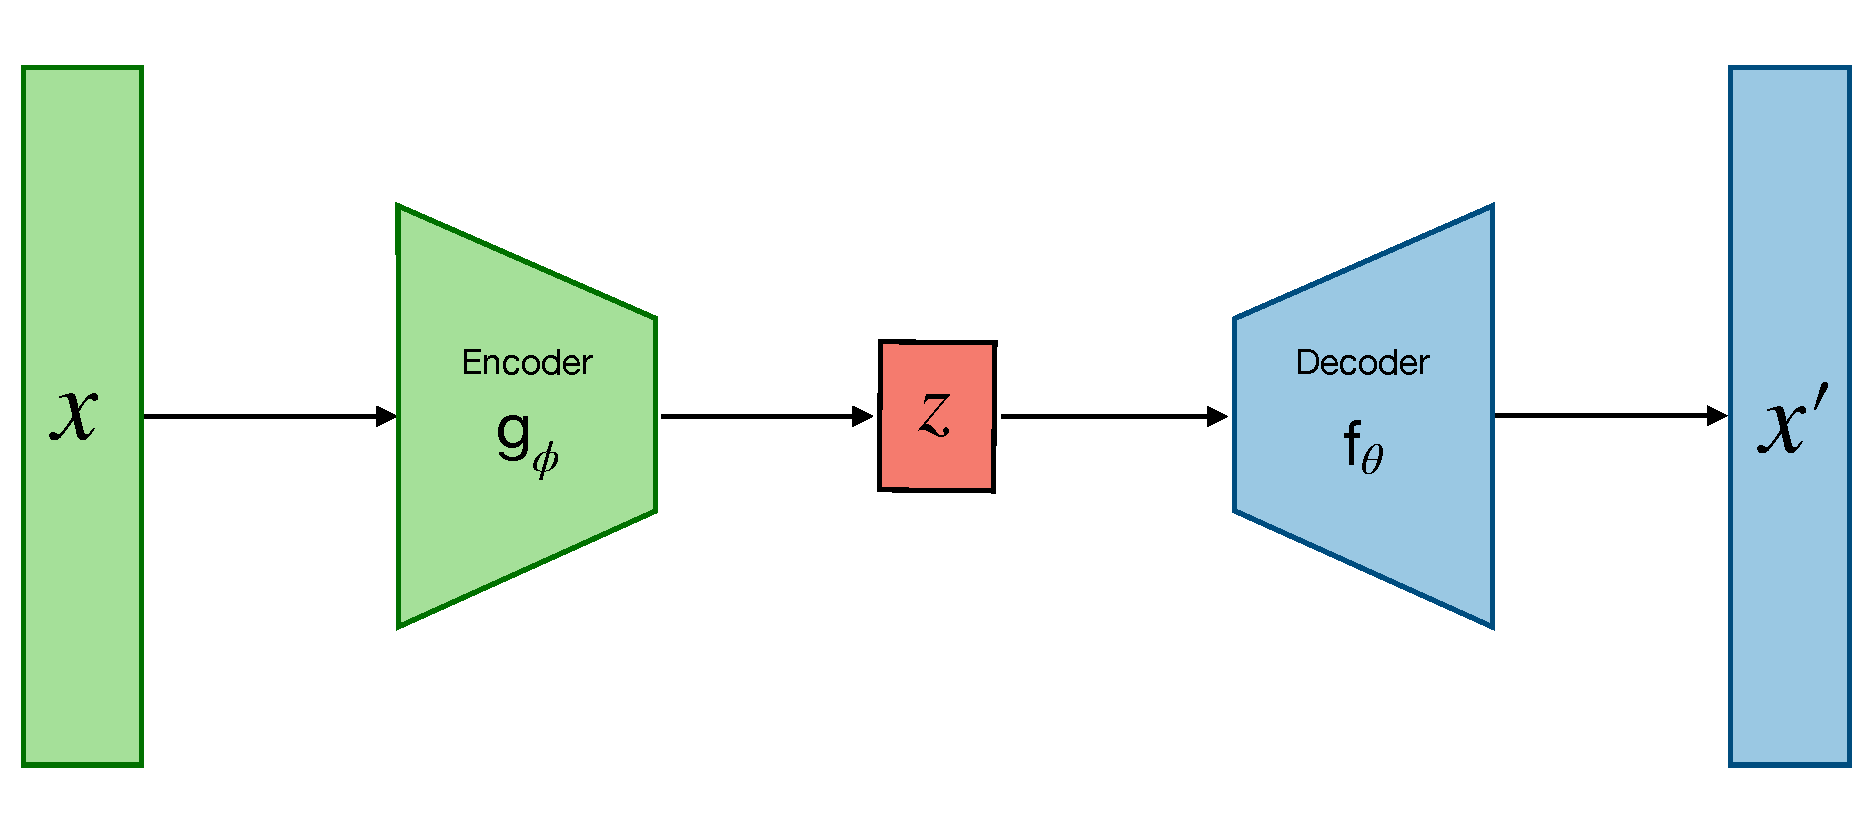
\includegraphics[width=\textwidth]{images/AE.pdf}
    \end{minipage}
    \hfill
    \begin{minipage}{0.7\textwidth}
        \centering
        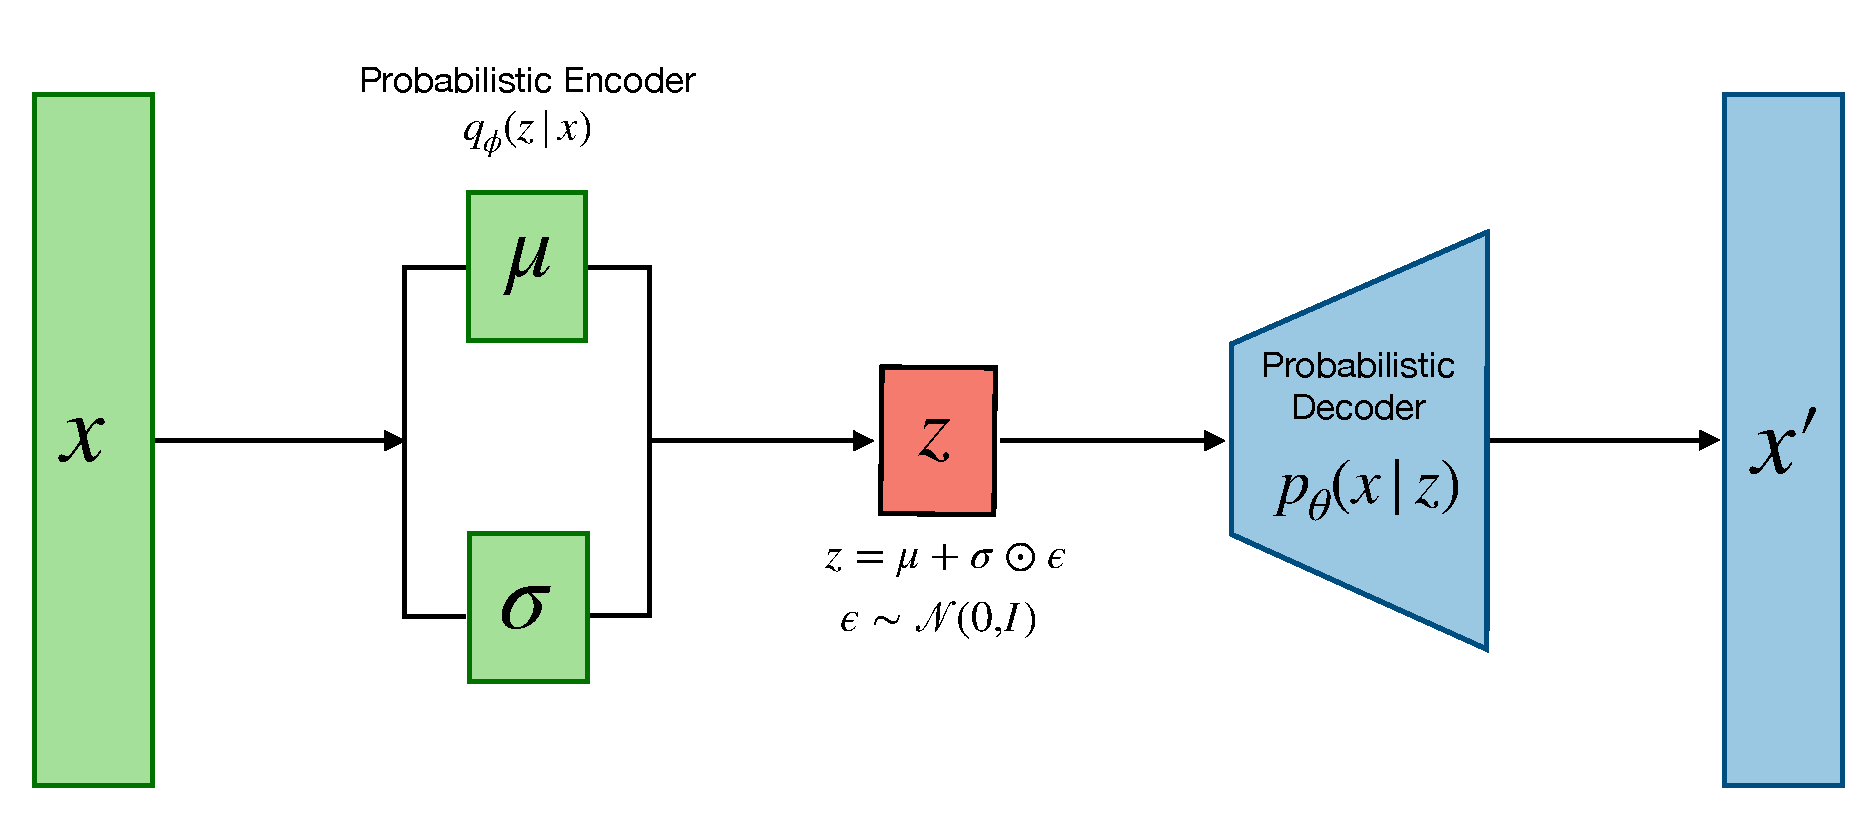
\includegraphics[width=\textwidth]{images/VAE.pdf}
    \end{minipage}
    \caption{Visual illustration of an Autoencoder (top) and a Variational Autoencoder (bottom). Inspired from 
    \cite{weng2018VAE}}
    \label{fig:AE_VAE}
\end{figure}


\subsection{Diffusion}
Diffusion models are a class of generative models that have gained significant attention 
for their ability to generate high-quality data (e.g., images, audio). These models 
operate by simulating two key processes: a forward diffusion process and a reverse 
denoising process.\newline
In the forward process, noise is gradually added to the data until it becomes indistinguishable
from a known distribution, typically Gaussian. The model then learns to reverse this process, 
step by step, denoising the data to recover samples that resemble those from the original dataset.\newline
A key difference between diffusion models and VAEs is that diffusion models operate through an iterative 
process, unlike VAEs which use a single step for encoding. Additionally, diffusion models 
do not reduce the dimensionality of the latent space and instead of learning the encoder they employ 
simple Gaussian noise as an encoder.
\vspace{-1cm}
\begin{figure}[H]
    \centering
    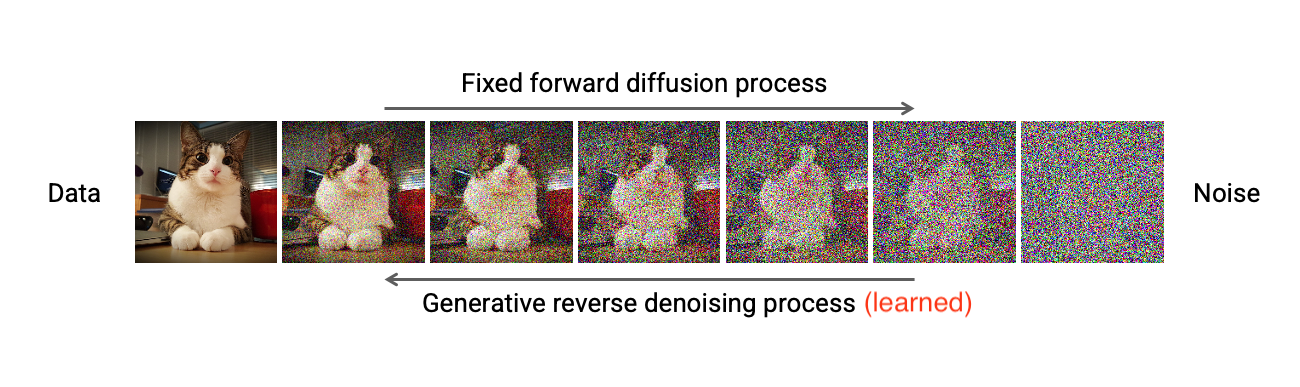
\includegraphics[width=1\linewidth]{images/diffusion.png}
    \caption{Illustration of the diffusion process}
    \label{fig:diffusion}
\end{figure}
The relationship between the data and latent variables in diffusion models is typically modeled as a Markov chain,
where each step depends only on the previous one.

\subsubsection{Forward Diffusion Process}
The forward diffusion process is a corruption process that takes a data sample (e.g., an 
image) and gradually adds noise to it in multiple steps, transforming the data into pure 
noise. This process can be described as follows:

\paragraph{Start with Data}
Start with an original data point $x_0$ (e.g., an image).

\paragraph{Add Noise in Steps}
At each time step $t$ noise is added to the previous state $z_{t-1}$ resulting in a more degraded version $z_t$. 
This process is modeled as a Markov chain:
\begin{align*}
    q(z_t | z_{t-1}) &= \mathcal{N}(z_t;\underset{\text{mean}}{\sqrt{1-\beta_t}z_{t-1}},\overset{\text{variance}}{\beta_tI}) \\
    &= \sqrt{1-\beta _t} z_{t-1} + \sqrt{\beta_t}\epsilon \sim \mathcal{N}(0,I) 
\end{align*}
We once again apply the reparameterization trick (see Section~\ref{reparametrization_trick}). 
To obtain $z_{100}$, the transformation would normally be applied sequentially over 100 steps. However, 
due to the properties of the Gaussian distribution, it is also possible to express this as a single-step
transformation from the original input. To do this, we define the following parameters:
$$\alpha_t = 1- \beta_t \qquad \bar{\alpha}_t = \prod_{s=1}^t\alpha_s$$ 
Here $\alpha_t$ defines the noise schedule, determining how much noise is added at each step. The one-step method can now be 
derived as follows:
\begin{align*}
    z_t &=  \sqrt{1-\beta _t} z_{t-1} + \sqrt{\beta_t} \epsilon \\
        &=  \sqrt{\alpha_t} {\color{cyan}z_{t-1}} + \sqrt{1-\alpha_t} \epsilon \\
        &=   \sqrt{\alpha_t} ({\color{cyan}\sqrt{\alpha_{t-1}} {\color{cyan}z_{t-2}} + \sqrt{1-\alpha_{t-1}} \epsilon}) + \sqrt{1-\alpha_t} \epsilon \numberthis \\
        &= \sqrt{\alpha_t \alpha_{t-1}}z_{t-2} +  
        \underbrace{\sqrt{\alpha_t-\alpha_t\alpha_{t-1}}\epsilon}_{\mathcal{N}(0,(\alpha_t-\alpha_t\alpha_{t-1})I)} + 
        \underbrace{\sqrt{1-\alpha_t} \epsilon}_{\mathcal{N}(0, (1-\alpha_t)I)} \\
        &=  \sqrt{\alpha_t \alpha_{t-1}}z_{t-2} + \sqrt{\alpha_t-\alpha_t\alpha_{t-1} + 1 - \alpha_t} \epsilon 
        &&(\text{sum of ind. gaussians \footnotemark})\\
        &= \sqrt{\alpha_{t}\alpha_{t-1}} z_{t-2} + \sqrt{1-\alpha_{t}\alpha_{t-1}}\epsilon \\
        &\vdots \quad (\text{repeat same steps from 14})\\
        &= \sqrt{\bar{\alpha}_t}z_0+\sqrt{1-\bar{\alpha}_t}\epsilon \\
        &\rightarrow q(z_t|z_0) = \mathcal{N}(z_t,\sqrt{\bar{\alpha}_t}z_0,\sqrt{1-\bar{\alpha}_t}I)
\end{align*}\footnotetext{Sum of two independent Gaussian variables $u \sim \mathcal{N}(\mu_u,\sigma_u^2)$ and 
$v \sim \mathcal{N}(\mu_v,\sigma_v^2)$ is a gaussian variable $ (u+v) \sim \mathcal{N}(\mu_u+\mu_v,\sigma_u^2+\sigma_v^2)$}

\subsubsection{Reverse Diffusion Process}
The reverse diffusion process is the key to generating new data points. It attempts to reverse the forward diffusion process 
and recover the original data from noise, essentially denoising the corrupted data step by step.
\paragraph{Start with Noise} The process starts with a noise sample, $z_t$, and iteratively denoises it by applying learned 
denoising steps.
\paragraph{Learned Model} The reverse process is learned by training a neural network to predict the denoised version 
of $z_t$ at each step $t$. Essentially, the model learns to reverse the noising process at each step meaning 
$p_\theta(z_{t-1}|z_t)$
\paragraph{Generate Data} By applying the reverse process step by step (starting from noise and gradually removing noise),
the model generates a new data sample that resembles the distribution of the original training data. The reverse process can 
be modelled as a parametrised Gaussian: 
$$p_\theta(z_{t-1}|z_t )= \mathcal{N}(z_{t-1};\mu_\theta(z_t,t),\Sigma_\theta(z_t,t))$$

\subsubsection{Training}
Training a diffusion model involves learning how to reverse the diffusion process. 
Specifically, the model is trained to predict the data at time step $t-1$ from the noisy 
data at time step $t$. This requires learning how to gradually denoise the data and 
requires a loss function that captures the reconstruction error over the multiple steps.
Diffusion models are trained using a likelihood-based approach, aiming to maximize the 
log-likelihood of the data. This is typically done through the Evidence Lower Bound (ELBO),
which incorporates various probabilistic components. A full derivation of this training objective
can be found in the original paper by Ho et al. \cite{ho2020denoisingdiffusionprobabilisticmodels}. 
The resulting bound is:
$$\log{p_\theta(x)} \geq \log{p_\theta(x|z_1)} - \overset{T}{\underset{t=2}{\sum}} \text{KL}(q(z_{t-1}|z_t,x)||p_\theta(z_{t-1}|z_t))-\text{KL}(q(z_T|x)||p(z_T))$$
This can be further simplified since the last term does not depend on the parameters 
$\theta$. Additionally, we know that $p_\theta(z_{t-1}|z_t)$  is the Gaussian we want to 
learn, and it turns out that  $q(z_{t-1}|z_t,x)$ is also a Gaussian. 
Therefore, we can use the closed-form KL divergence between two Gaussians. 

%\begin{figure}[H]
%\begin{minipage}[t]{0.495\textwidth}
%\begin{algorithm}[H]
%  \caption{Training} \label{alg:training}
%  \small
%  \begin{algorithmic}[1]
%    \REPEAT
%      \STATE $x_0 \sim q(x_0)$
%      \STATE $t \sim \mathrm{Uniform}(\{1, \dotsc, T\})$
%      \STATE $\epsilon\sim\mathcal{N}(0,I)$
%      \STATE Take gradient descent step on
%      \STATE $\qquad \nabla_\theta \left\| \epsilon - \epsilon_\theta(\sqrt{\bar\alpha_t} x_0 + \sqrt{1-\bar\alpha_t}\epsilon, t) \right\|^2$
%    \UNTIL{converged}
%  \end{algorithmic}
%\end{algorithm}
%\end{minipage}
%\hfill
%\begin{minipage}[t]{0.495\textwidth}
%\begin{algorithm}[H]
%%  \caption{Sampling} \label{alg:sampling}
%  \small
%  \begin{algorithmic}[1]
%    \vspace{.04in}
%    \STATE $x_T \sim \mathcal{N}(0, I)$
%    \FOR{$t=T, \dotsc, 1$}
%      \STATE $z \sim \mathcal{N}(0, I)$ if $t > 1$, else $z = 0$
%      \STATE $x_{t-1} = \frac{1}{\sqrt{\alpha_t}}\left( x_t - \frac{1-\alpha_t}{\sqrt{1-\bar\alpha_t}} \epsilon_\theta(x_t, t) \right) + \sigma_t z$
%    \ENDFOR
%    \STATE \textbf{return} $x_0$
%    \vspace{.04in}
%  \end{algorithmic}
%\end{algorithm}
%\end{minipage}
%\vspace{-1em}
%\end{figure}

\subsection{Score-Based Generative Models}
Score-based generative models \cite{song2021scorebasedgenerativemodelingstochastic} are a class of models that learn
the score function of a data distribution — the gradient of the log-probability density with respect to the data:
$$\nabla_x \log{p(x)}$$
As with other generative models, the goal is to learn the data distribution $p_\theta(x)$ and generate new samples from it.
A common formulation expresses the data distribution as:
$$p_\theta(x) = \frac{e^{-f_\theta(x)}}{Z_\theta}$$
However, the problem with this direct approach is that it requires knowledge of the 
normalization constant $Z_\theta$, which involves solving an integral over the entire 
domain, a task that is often intractable. By instead taking the gradient of the log-probability, we get:
$$\nabla_x \log{p_\theta(x)} = \nabla_x \log{e^{-f_\theta(x)}}-\nabla_x \log{Z_\theta}=- \nabla_x f_\theta(x)$$
This is the core insight of score-based models: instead of modeling $p_\theta(x)$ directly, we model how the probability 
density changes in space. Once the score function is learned, we can generate samples by following these gradients in a 
stochastic manner (e.g., via Langevin dynamics).

\subsection{Flow Matching}
Flow matching \cite{lipman2023flowmatchinggenerativemodeling} is a method for training generative models based on 
the idea of aligning data distributions through normalizing flows. A normalizing flow is a series of invertible
transformations applied to a simple distribution (e.g., a Gaussian) to model complex data distributions.\newline
Flow matching introduces a novel way of training generative models by matching the gradients of the data density 
at different stages of the transformation. This is done by learning the flow that transforms a simple distribution 
(like Gaussian noise) into a more complex data distribution.
Really helpful resource can be found \href{https://www.youtube.com/watch?v=7cMzfkWFWhI}{here}


\subsection{Connecting Diffusion Models and Reinforcement Learning}
An interesting connection exists between diffusion models and reinforcement learning (RL): diffusion models can be used to 
generate new plausible policies that resemble those from the original dataset. In other words, instead of learning from the 
dataset directly, we learn a distribution over good trajectories (or policies), and then sample new ones using diffusion 
processes. This perspective opens up new possibilities in offline RL and imitation learning, where the goal is to generalize 
and generate diverse, high-performing behaviors from limited data.

\subsection{Resources}
In this section, we did not delve into the full mathematical derivations behind the various generative modeling approaches, as 
these tend to be quite lengthy. For readers interested in the detailed math, I recommend reading the original papers. 
Additionally, there are some excellent resources that explain these concepts more intuitively. A great video series covering 
diffusion models, score-based diffusion models, and flow matching can be found here \cite{outlier}. Lilian Weng’s blog post "What 
Are Diffusion Models?" \cite{weng2021diffusion} is also very well written and highly recommended. For a deeper understanding of 
score-based models, Yang Song’s blog \cite{YangSong} is one of the best resources available. A particularly insightful paper that 
highlights the connections between the various generative modeling approaches discussed is \cite{luo2022understandingdiffusionmodelsunified}.

